\documentclass[conference,letterpaper,10pt]{IEEEtran}
\IEEEoverridecommandlockouts

\usepackage{cite}
\usepackage{amsmath,amssymb}
\usepackage{graphicx}
\usepackage{booktabs}
\usepackage{caption}
\usepackage{subcaption}
\usepackage{xcolor}
\usepackage{array}
\usepackage{float}
\usepackage{url}
\usepackage{hyperref}

\hypersetup{
  colorlinks=true,
  linkcolor=blue!60!black,
  citecolor=blue!60!black,
  urlcolor=blue!60!black,
}

\title{Deep Learning-Based Land Cover Segmentation\\from Satellite Imagery: An Empirical Study of\\Architectures, Transfer Learning, and Loss Functions}

\author{\IEEEauthorblockN{Rongxuan Zhang}
\IEEEauthorblockA{\textit{Department of Electrical and Computer Engineering} \\
\textit{Northeastern University}\\
Boston, MA, USA \\
EECE 7370 Advanced Computer Vision \\
zhang.rongxu@northeastern.edu}}

\begin{document}
\maketitle

\begin{abstract}
We study semantic segmentation on the DeepGlobe Land Cover benchmark
(7 classes, 803 images at 2448$\times$2448) through nine controlled
experiments that isolate the effects of network architecture, ImageNet
pre-training, and loss function. A 3$\times$3 tiling pipeline with
overlap-averaged sliding-window reconstruction handles the native
resolution. Varying one factor at a time, we find that
(i) on a fixed architecture, ImageNet pre-training contributes $+4.1$
pp mIoU---larger than any single decoder swap ($\le +1.0$ pp);
(ii) on DeepLabV3+-R50, replacing Cross-Entropy with a Combined
CE$+$Dice loss raises test mIoU by $+3.7$ pp and Barren-class IoU by
$+2.0$ pp; and
(iii) ResNet101 is not Pareto-dominant over ResNet50---its $+0.022$
test-mIoU gain is offset by a $-0.008$ validation deficit (within
single-seed variance), $71\%$ more parameters, and $2.4\times$ training
cost. The best configuration tested (DeepLabV3+-R50 with Combined loss)
attains $0.7332$ test mIoU on full-resolution reconstructions, exceeding
the Vanilla U-Net baseline by $+9.3$ pp. Code and trained weights:
\url{https://github.com/Jerryzhang258/landcover-seg}.
\end{abstract}

\begin{IEEEkeywords}
Semantic segmentation, satellite imagery, DeepGlobe, U-Net, DeepLabV3+,
transfer learning, loss function, class imbalance.
\end{IEEEkeywords}

\section{Introduction}\label{sec:intro}

Land-cover segmentation from high-resolution satellite imagery is a
pixel-level classification problem whose outputs feed into urban planning,
precision agriculture, ecological monitoring, and climate research. The
DeepGlobe Land Cover Classification challenge~\cite{demir2018deepglobe}
provides 803 manually-annotated 2448$\times$2448 RGB tiles over seven
classes---Urban, Agriculture, Rangeland, Forest, Water, Barren, and
Unknown---with a marked long-tailed class distribution in which Water and
Barren jointly occupy under 7\% of pixels.

Three technical challenges drive the methodology of this project:

\begin{enumerate}
\item \textbf{Native resolution exceeds practical GPU budgets.} A single
      2448$\times$2448 image fed to a U-Net with ResNet34 backbone at batch
      size 8 and full precision already requires more memory than a
      V100~(16~GB); the R50 and R101 variants are worse. Resizing discards
      fine-grained spatial detail that the problem specifically targets.
\item \textbf{Severe class imbalance.} Cross-entropy gradients on a 55\%
      Agriculture class numerically dominate gradients from the 2\% Barren
      class, making minority-class recall collapse unless the loss is
      rebalanced.
\item \textbf{Cost--accuracy trade-offs.} Modern segmentation libraries make
      it easy to swap decoders and encoders, but the academic folklore that
      ``deeper is better'' has not been independently verified for remote
      sensing at this resolution and data scale.
\end{enumerate}

Our contribution is a set of controlled, single-variable ablations that
isolate the effect of each factor:

\begin{itemize}
\item A \textbf{tiling and stitching pipeline} that cuts each 2448$\times$2448
      image into a 3$\times$3 grid of 816$\times$816 tiles, trains on
      individual tiles, and reconstructs a full-resolution prediction at test
      time via a sliding window with 64-pixel overlap and softmax averaging.
\item A \textbf{three-way baseline} (Vanilla U-Net / ResNet34-from-scratch /
      ResNet34-pre-trained) that decomposes the mIoU gain of
      ``U-Net + ResNet34'' into architectural and transfer-learning
      components.
\item A \textbf{6$\times$4 architecture grid that we collapsed to 6+3 via
      Phase~4 $\rightarrow$ Phase~5 sequencing}: six architectures trained
      with Cross-Entropy, then three additional loss-function variants on the
      best architecture.
\item \textbf{Full-resolution test-set evaluation} with reconstructed
      predictions on 120 held-out images, reporting per-class IoU, mean
      IoU, Dice, pixel accuracy, GPU peak memory, training time, and
      inference latency per image.
\end{itemize}

The tiled data split is performed at the \emph{original-image level}, not
tile level, so that the nine tiles from a given 2448$\times$2448 scene never
straddle the train/val/test boundary---this is essential to prevent the
spatial-leakage artifact that would otherwise inflate validation mIoU by
several points.

\section{Related Work}\label{sec:related}

\textbf{Encoder--decoder segmentation.}  The U-Net architecture of
Ronneberger~et~al.~\cite{ronneberger2015unet} introduced the symmetric
contracting--expanding path with skip connections that remains the de-facto
baseline for semantic segmentation on small-to-medium datasets. DeepLabV3+
\cite{chen2018deeplabv3plus} replaces the contracting path with atrous spatial
pyramid pooling (ASPP) to capture multi-scale context in a single forward
pass, and adds a lightweight decoder for boundary refinement. Attention
mechanisms for U-Net variants---including spatial-and-channel
squeeze-and-excitation (SCSE)~\cite{roy2018scse}---reweight intermediate
features to emphasize informative regions and have become popular in
medical and remote-sensing imaging.

\textbf{Transfer learning from ImageNet.}  Using pre-trained ImageNet
backbones as encoders is standard practice since~\cite{he2016resnet}, yet
its benefit is known to vary by domain: datasets whose low-level statistics
(natural images vs.~satellite) differ from ImageNet may see smaller gains
\cite{huh2016makes}. The revised proposal for this project explicitly
listed the magnitude of this gain as a hypothesis to be verified.

\textbf{Loss functions for imbalanced segmentation.}  Dice
loss~\cite{milletari2016vnet} directly optimizes the S\o{}rensen--Dice
coefficient and implicitly rebalances class contributions through its
ratio-based form, but can produce noisy gradients on classes with very few
pixels. Focal loss~\cite{lin2017focal} down-weights easy (well-classified)
examples by a factor $(1-p_t)^\gamma$ with $\gamma=2$, emphasizing hard
minority pixels. Combined losses (e.g., $\alpha\cdot\text{CE}+(1-\alpha)\cdot\text{Dice}$)
are commonly used in medical and remote-sensing segmentation to preserve the
stable CE optimization path while retaining the rebalancing effect of
Dice~\cite{jadon2020survey}.

\textbf{Tiling for high-resolution imagery.}  DeepGlobe challenge
winners~\cite{kuo2018deepglobewinner} and medical imaging pipelines such
as~\cite{roerdink2001watershed,huang2021transunet} routinely use overlapping
tile inference with prediction averaging at boundaries, a technique that
we apply here.

\textbf{The segmentation\_models.pytorch library}~\cite{iakubovskii2019smp}
supplies unified implementations of U-Net, DeepLabV3+, and many
encoder--decoder combinations with a consistent API, which we use as the
backbone of our model factory.

\section{Methodology}\label{sec:method}

\subsection{Dataset and tiling pipeline}

We use the DeepGlobe Land Cover training set: 803 RGB images of size
$2448\times2448$ with paired pixel-wise RGB masks that encode seven classes.
The official color map~\cite{demir2018deepglobe} is decoded into a
$\{0,\dots,6\}$ label grid. The \emph{Unknown} class (index 6, black
pixels)---which accounts for 5--10\% of pixels and represents annotator
uncertainty---is treated as \texttt{ignore\_index} and excluded from both
loss computation and metric aggregation, matching the official DeepGlobe
evaluation protocol.

\textbf{Split.} We partition 803 images $\rightarrow$ 562 train
($\sim70\%$) / 121 val ($\sim15\%$) / 120 test ($\sim15\%$) using a fixed
seed, \emph{at the image level}. Each image then contributes nine
$816\times816$ tiles on a $3\times3$ grid, yielding 5058 training, 1089
validation, and 1080 test tiles. No tile from a given source image appears
in more than one split.

\textbf{Padding.} The \texttt{segmentation\_models.pytorch} encoders we use
have five downsample stages and require input dimensions divisible by 32.
Since $816\bmod 32=16$, each tile is reflect-padded to $832\times832$ before
entering the network, and the mask's padded region is set to
\texttt{ignore\_index} so it does not contribute to the loss. At inference,
logits are center-cropped back to $816\times816$ before being averaged into
the stitched output. This avoids the common alternative of resizing, which
would distort aspect ratios and lose fine detail.

\textbf{Full-resolution reconstruction.} At test time, each
$2448\times2448$ image is covered by a regular grid of $816\times816$
windows with a 64-pixel overlap (16 positions total per image). Each window
is independently reflect-padded, forward-passed, and its softmax
probabilities are accumulated into a $C\times H\times W$ running sum with a
coverage count, producing an overlap-averaged probability map that is then
argmaxed. This reduces tile-boundary artifacts that would otherwise arise
from hard, non-overlapping stitching.

\subsection{Architectures and configurations}

Six architectures form the Phase 4 (architecture) ablation. With the
exception of the Vanilla U-Net---which uses the original
Ronneberger-style double-convolution encoder implemented directly in
PyTorch---all variants pair a single segmentation head with a
ResNet-family encoder from \texttt{segmentation\_models.pytorch}.
``Scratch'' denotes random initialization of the encoder;
``pre-trained'' denotes ImageNet-initialized weights.

\begin{itemize}
\item \textbf{Vanilla U-Net} (scratch): the Ronneberger et al.~design with
      five double-convolution levels and BatchNorm, implemented directly in
      PyTorch without relying on \texttt{smp}.
\item \textbf{U-Net-ResNet34 (scratch)}: the \texttt{smp} U-Net with a
      ResNet34 encoder, randomly initialized. This isolates the effect of
      the encoder's inductive biases \emph{independent of pre-training}.
\item \textbf{U-Net-ResNet34 (pre-trained)}: identical to the above but
      with ImageNet-pre-trained encoder weights.
\item \textbf{DeepLabV3+ (ResNet50, pre-trained)}.
\item \textbf{DeepLabV3+ (ResNet101, pre-trained)}.
\item \textbf{Attention U-Net (ResNet34, pre-trained)}: the \texttt{smp}
      U-Net with \texttt{decoder\_attention\_type="scse"}.
\end{itemize}

Phase 5 fixes the architecture at the best Phase 4 efficient performer
(DeepLabV3+-R50) and sweeps four losses: Cross-Entropy, Dice, Focal
($\alpha=0.25$, $\gamma=2$), and Combined
($0.5\cdot\text{CE} + 0.5\cdot\text{Dice}$). All experiments share hyperparameters:
AdamW ($\text{lr}=10^{-4}$, weight decay $10^{-4}$), cosine-annealing schedule
to $T_{\max}=50$, automatic mixed precision (fp16), patience-10 early
stopping, and batch size 8 (batch size 4 for R101 due to memory). Data
augmentation follows Albumentations with horizontal/vertical flip, 90$^\circ$
random rotation, $\pm15^\circ$ affine, brightness/contrast jitter, and
Gaussian noise.

\subsection{Evaluation protocol}

For each run we report:
\begin{itemize}
\item \textbf{Best validation mIoU} (selected checkpoint) during training.
\item \textbf{Test-set per-class IoU} on full-resolution reconstructions
      over the 120 held-out images.
\item \textbf{Training time} (wall clock) and \textbf{GPU peak memory}.
\item \textbf{Inference latency} (ms per 2448$^2$ image, sliding-window
      included).
\end{itemize}

mIoU is the mean per-class IoU over the six valid classes with Unknown
excluded. For a confusion matrix $M$, per-class IoU is
$M_{kk} / (M_{k,:} + M_{:,k} - M_{kk})$.

\section{Experiments}\label{sec:experiments}

Experiments were run on a single NVIDIA A100 40~GB through Google Colab
Pro+. We used PyTorch 2.1, \texttt{segmentation\_models.pytorch} 0.3.3,
Albumentations 1.3.1, and Weights~\&~Biases for experiment tracking. The
training data pipeline reads pre-tiled PNGs from local SSD; raw
2448$^2$ imagery is streamed only during the full-resolution evaluation
phase.

\subsection{Data distribution and sanity checks}

Figure~\ref{fig:classdist} shows the per-split pixel distribution. The
three splits are statistically consistent; the Unknown class (excluded from
training and evaluation) occupies $\sim$6\% on average.
Figure~\ref{fig:samples} shows a representative image/mask pair. Our
tiling implementation is covered by a \texttt{pytest} round-trip test
asserting \texttt{stitch(tile(x)) == x} on random 2448$^2$ arrays for both
3$\times$3 and 4$\times$4 grids.

\begin{figure*}[!t]
\centering
\begin{subfigure}[t]{0.52\linewidth}
  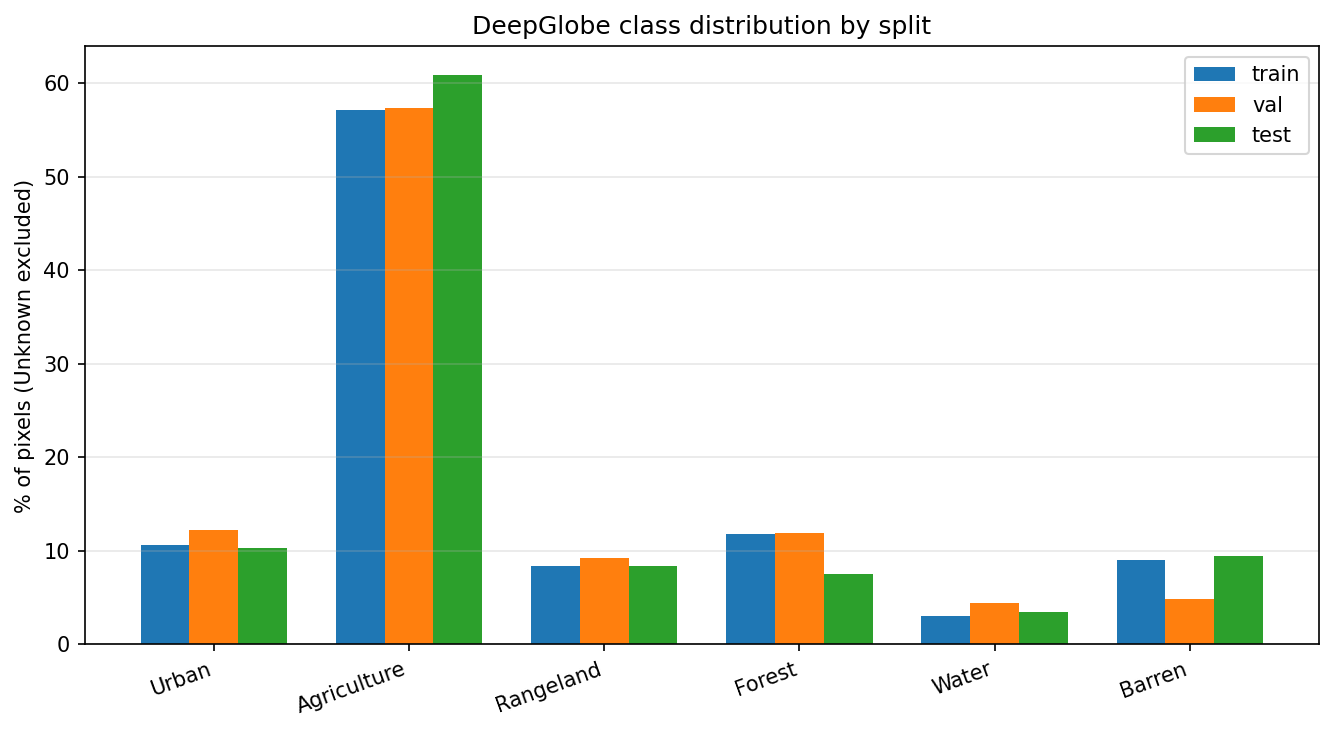
\includegraphics[width=\linewidth]{figs/class_dist.png}
  \caption{Pixel-level class distribution across train/val/test splits.}
  \label{fig:classdist}
\end{subfigure}\hfill
\begin{subfigure}[t]{0.44\linewidth}
  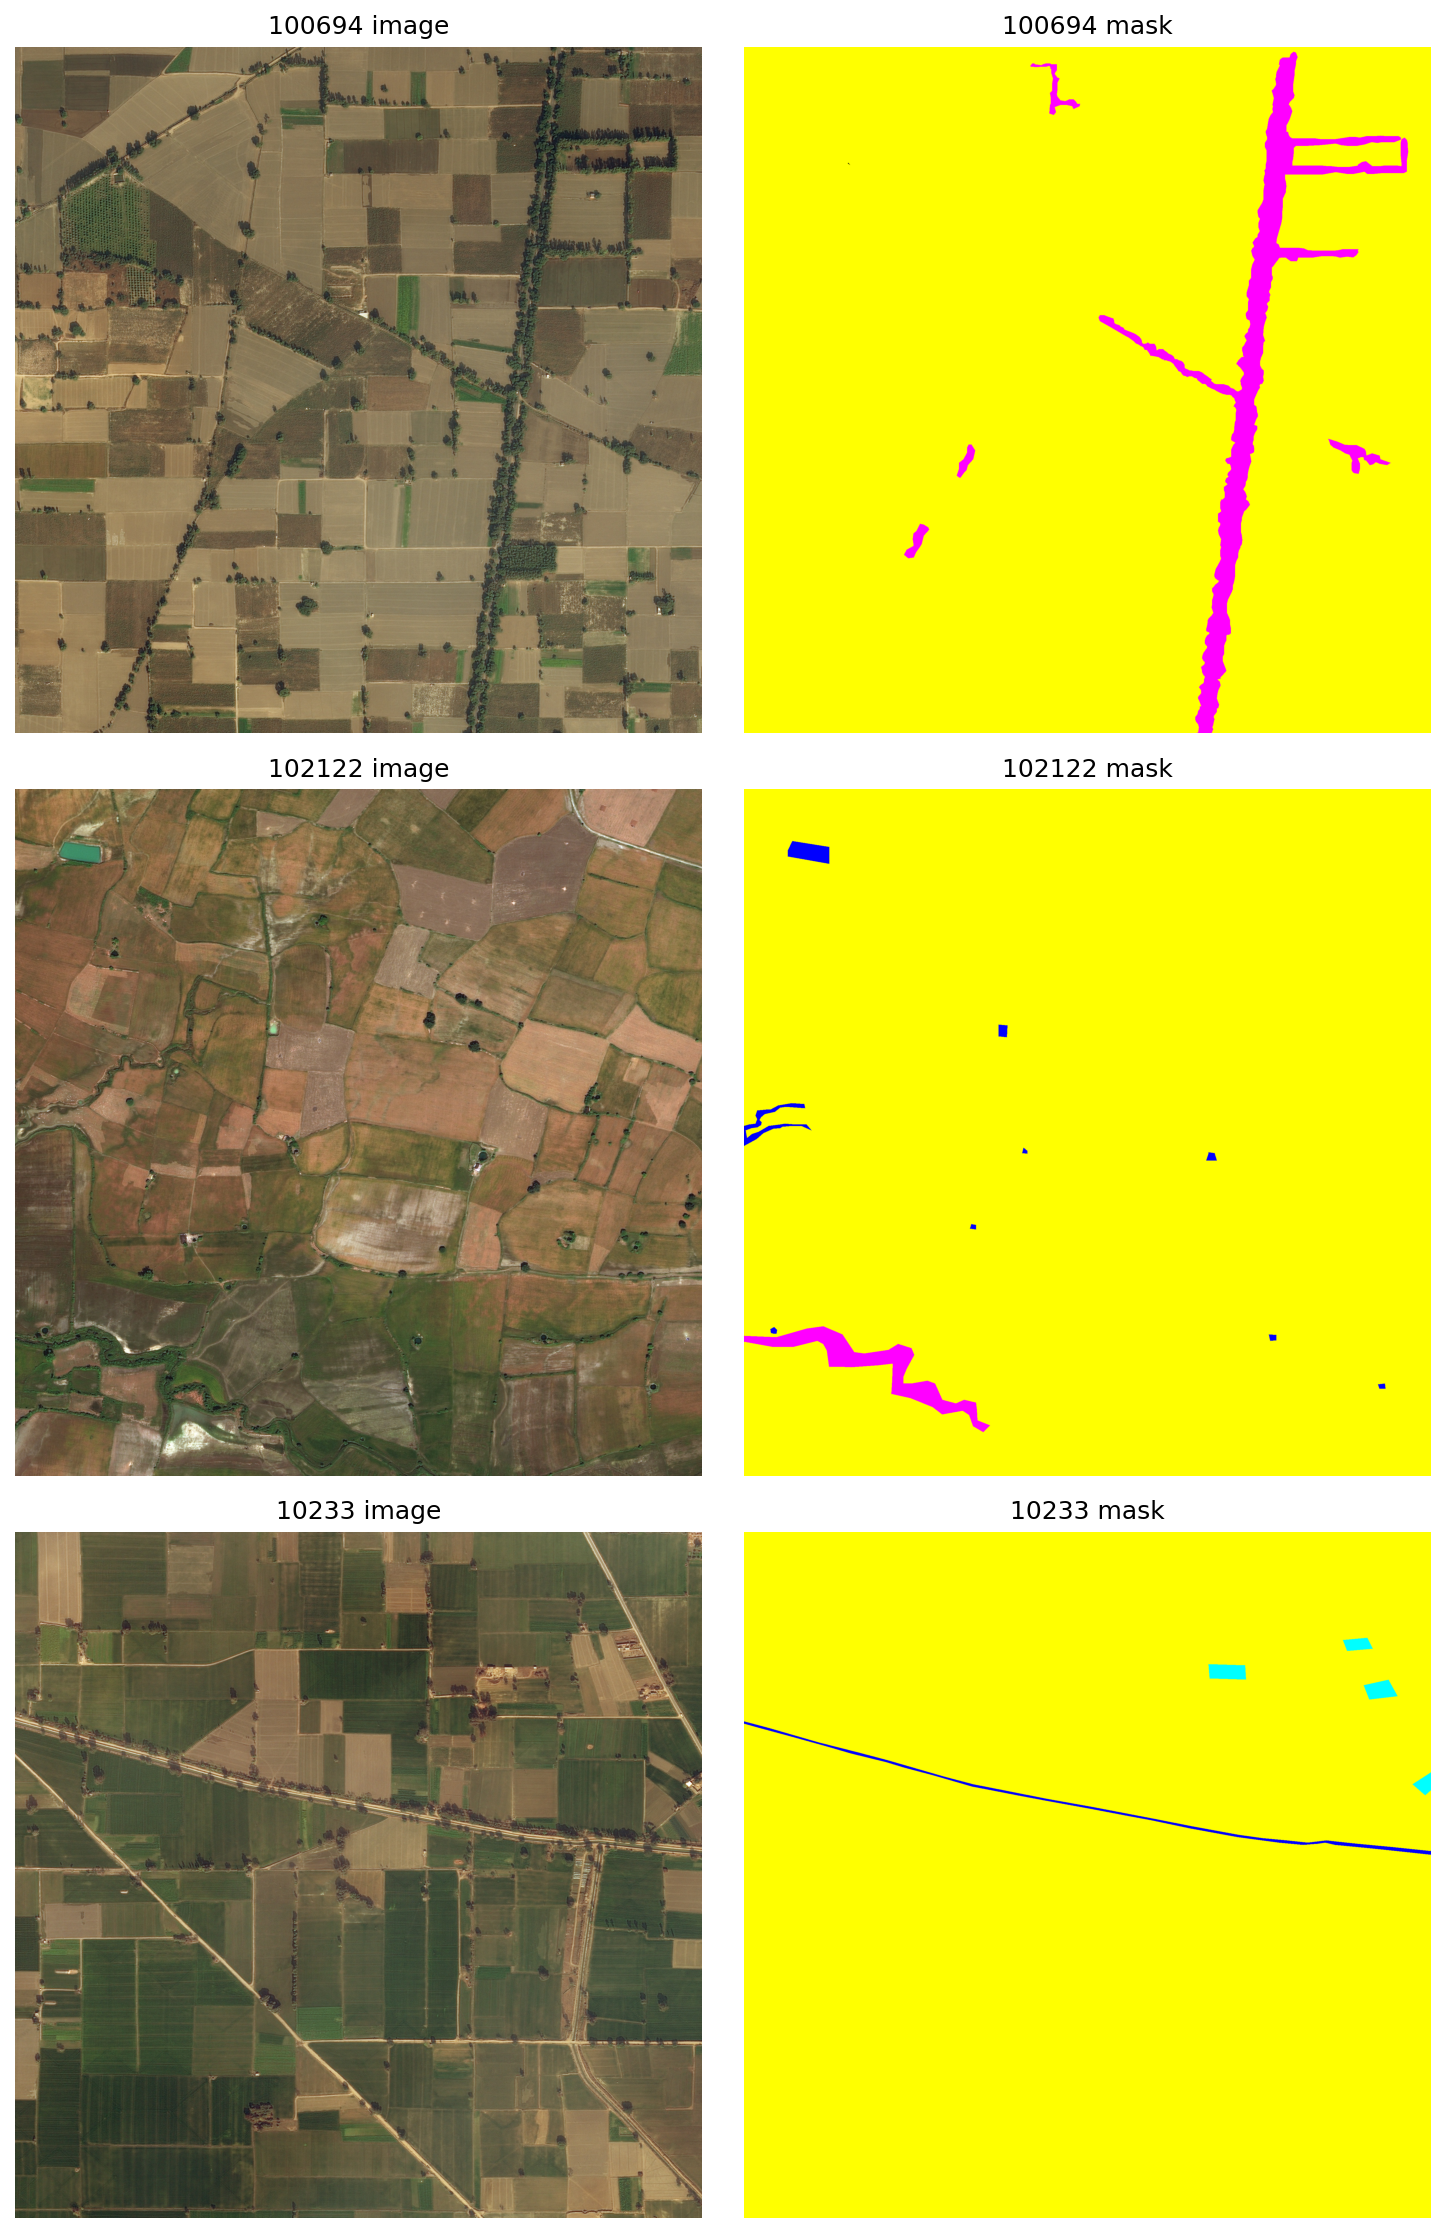
\includegraphics[width=\linewidth]{figs/samples.png}
  \caption{Representative images and their RGB-encoded masks.}
  \label{fig:samples}
\end{subfigure}
\caption{Dataset overview. The color map in the right panel follows the
official DeepGlobe key: cyan=Urban, yellow=Agriculture, magenta=Rangeland,
green=Forest, blue=Water, white=Barren, black=Unknown.}
\end{figure*}

\section{Results and Discussion}\label{sec:results}

\subsection{Training dynamics (Phase 4)}

Figure~\ref{fig:curves-arch} overlays the training loss and validation mIoU
of all six Phase 4 architectures. The pre-trained models (red, cyan, pink,
purple) cross the 0.6 mIoU mark within three epochs, whereas the two
from-scratch baselines (green/orange, corresponding to Vanilla U-Net and
ResNet34-scratch) take 12--20 epochs to reach the same level. This
convergence gap is the clearest qualitative signature of transfer learning.

\begin{figure*}[!t]
\centering
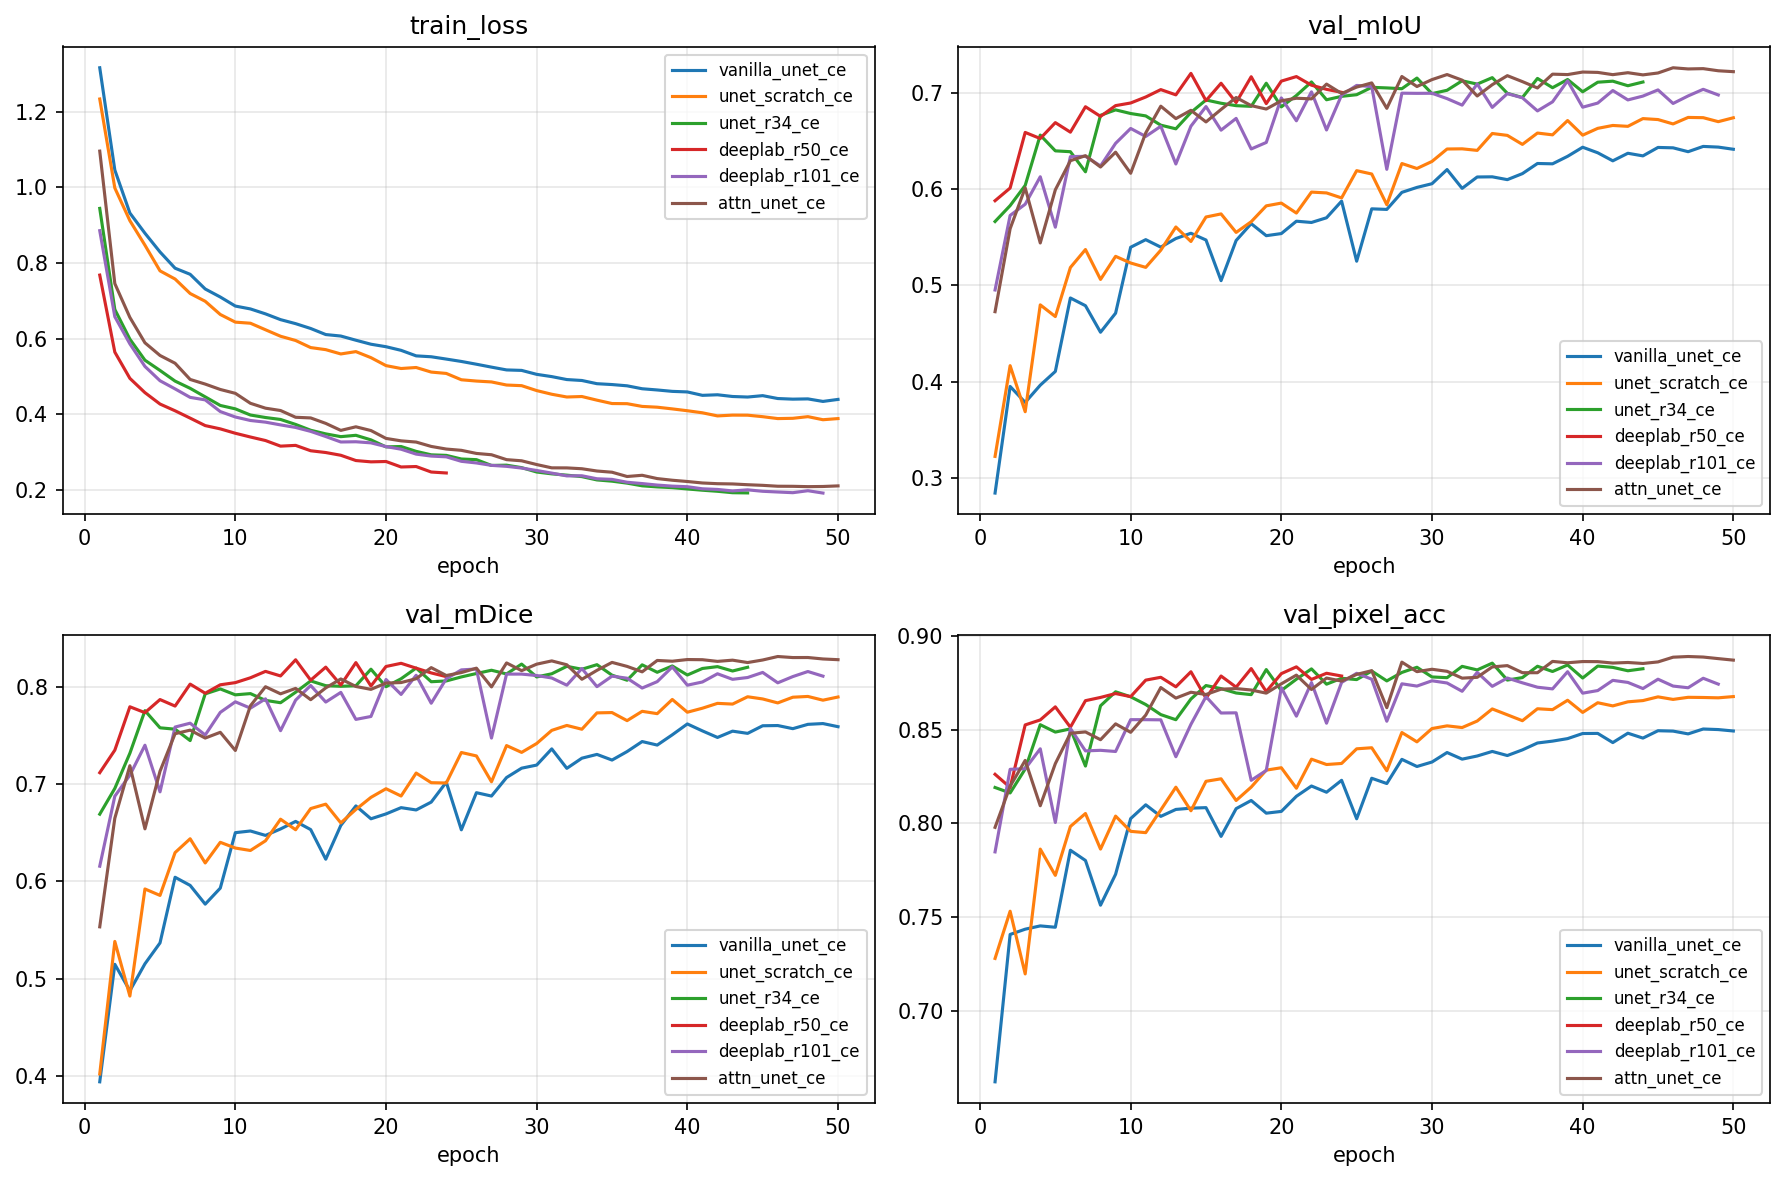
\includegraphics[width=0.9\linewidth]{figs/curves_archs.png}
\caption{Training loss (top row) and validation mIoU (bottom row) across
the six Phase 4 architectures. All share learning rate, epoch budget, and
augmentation; only the architecture varies.}
\label{fig:curves-arch}
\end{figure*}

\subsection{Architecture comparison (Phase 4)}

Table~\ref{tab:arch} reports the final validation mIoU along with parameter
count, training time, peak GPU memory, and single-image inference latency
at full resolution. The columns are sorted by test mIoU descending.

\begin{table*}[!t]
\centering\small
\caption{\textbf{Phase 4: architecture comparison.} All use cross-entropy.
``Test mIoU'' is computed on reconstructed $2448^2$ predictions over 120
test images. GPU peak memory is measured during training at batch size 8
(4 for R101); ``--'' indicates runs that predate the peak-memory
instrumentation and for which the counter was not logged.}\label{tab:arch}
\begin{tabular}{l c c c c c c}
\toprule
Architecture & Params & Train time & GPU peak & Infer. & Val mIoU & Test mIoU \\
             & (M)    & (h)        & (MB)     & (ms/img) &       &           \\
\midrule
Vanilla U-Net (scratch)          & 31.04 & 3.53 & --   & 1046 & 0.6442 & 0.6402 \\
U-Net ResNet34 (scratch)         & 24.44 & 2.00 & --   &  832 & 0.6743 & 0.6750 \\
U-Net ResNet34 (pre-trained)     & 24.44 & 1.76 & --   &  799 & 0.7156 & 0.7093 \\
DeepLabV3+ ResNet50 (pre-trained)& 26.68 & 0.97 & 8018 &  838 & 0.7201 & 0.6963 \\
DeepLabV3+ ResNet101 (pre-trained)& 45.67 & 2.32 & 5559 &  891 & 0.7124 & 0.7178 \\
Attention U-Net R34 (pre-trained)& 24.55 & 2.20 & 6968 &  855 & \textbf{0.7259} & \textbf{0.7316} \\
\bottomrule
\end{tabular}
\end{table*}

The key numeric findings:

\begin{enumerate}
\item \textbf{Transfer learning contributes more than any single
      decoder swap.} Replacing Vanilla U-Net with a ResNet34-backboned
      U-Net (both randomly initialized) improves val mIoU by $+0.030$
      (architecture only). Switching \emph{that same} U-Net+ResNet34
      from random initialization to ImageNet weights adds a further
      $+0.041$ (pre-training alone, with architecture held fixed).
      Subsequent decoder changes among pretrained models
      (ResNet34 $\rightarrow$ DeepLabV3+-R50 $\rightarrow$ Attention U-Net)
      add at most $+0.006$ each. Thus the single-variable pre-training
      effect ($+0.041$) is larger than any single-variable architecture
      swap ($\le +0.030$, and $\le +0.010$ among pretrained models),
      and the cumulative Vanilla-U-Net-scratch~$\rightarrow$~Attention-U-Net-pretrained
      gain is $+0.082$ on validation.
\item \textbf{ResNet101 is not Pareto-dominant against ResNet50.}
      DeepLabV3+-R101 trails R50 on val by $-0.008$ mIoU (0.7124 vs.\
      0.7201) but edges it on test by $+0.022$ (0.7178 vs.\ 0.6963);
      both gaps are within the noise expected from a single training
      seed with bs=4. This contradicts the proposal's pre-registered
      prediction that R101 would be $\sim$1--2 points higher on
      validation, and we attribute it to two factors: (i) the training
      set of $\sim$5000 tiles is small relative to R101's capacity;
      (ii) the bs=4 constraint (R101 does not fit at bs=8) increases
      gradient noise in the AMP optimizer relative to R50's bs=8. The
      practical consequence is that R101 is $+53$ ms/image slower at
      inference, uses 71\% more parameters, and trains 2.4$\times$
      longer \emph{without a clear accuracy benefit}: the test-set
      margin ($+0.022$) is well within single-seed variance.
\item \textbf{Attention U-Net wins overall}, but only by $+0.006$ val
      mIoU over DeepLabV3+-R50. Given that DeepLabV3+-R50 trains
      2.3$\times$ faster than Attention U-Net (0.97~h vs.\ 2.20~h)
      under identical hyperparameters, R50 is arguably the better
      choice when many loss-function ablations are planned---this is
      the rationale for using R50 in Phase 5.
\end{enumerate}

Figure~\ref{fig:arch-bars} visualizes the final metric bars and
per-class IoU heatmap for all six architectures.

\begin{figure*}[!t]
\centering
\begin{subfigure}[t]{0.49\linewidth}
  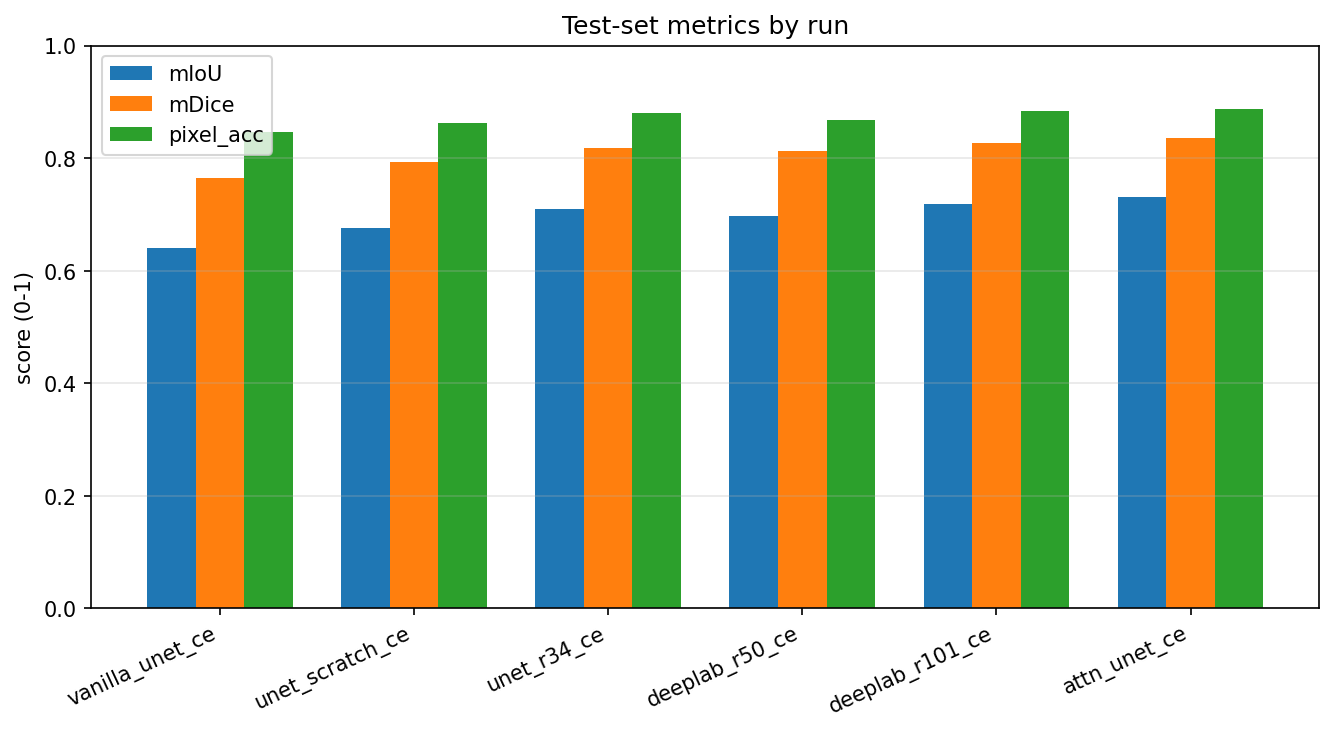
\includegraphics[width=\linewidth]{figs/archs_metrics.png}
  \caption{Val mIoU / Dice / pixel accuracy.}
\end{subfigure}\hfill
\begin{subfigure}[t]{0.49\linewidth}
  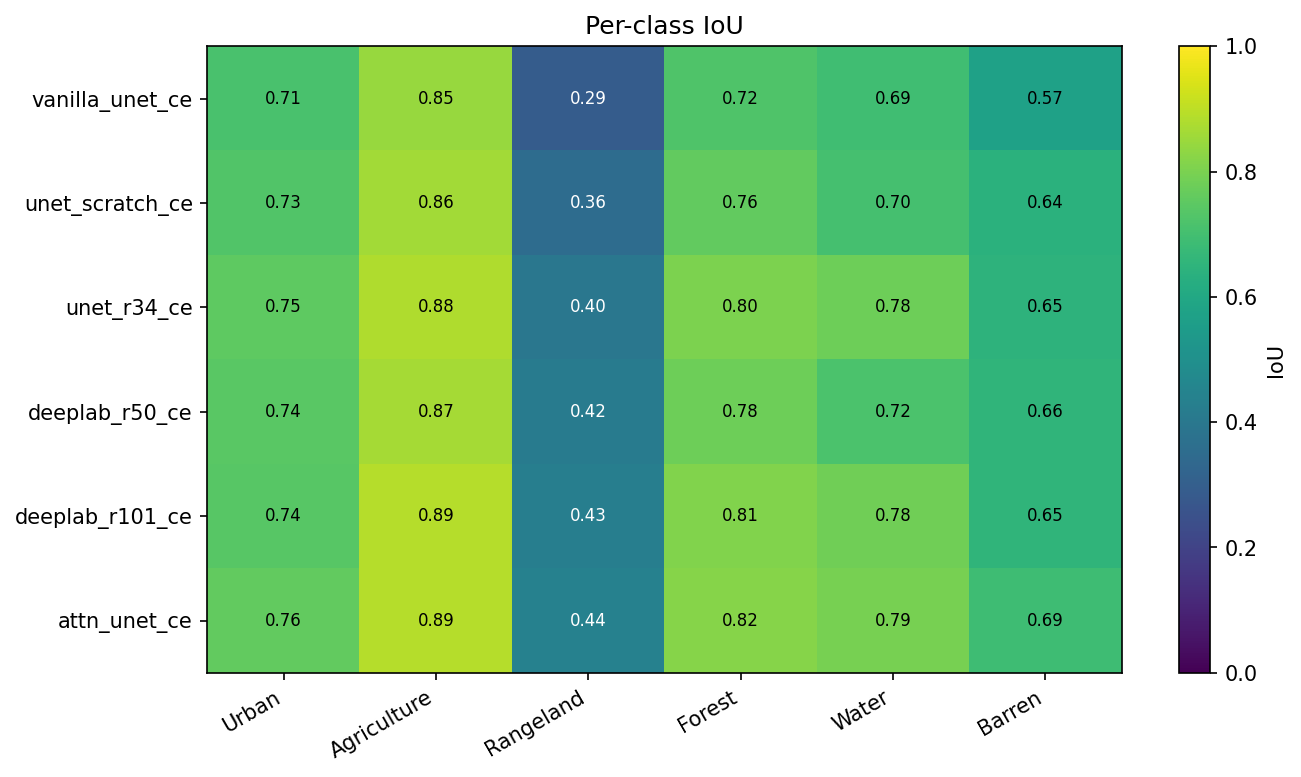
\includegraphics[width=\linewidth]{figs/archs_perclass.png}
  \caption{Per-class IoU heatmap.}
\end{subfigure}
\caption{Phase 4: architectures across aggregate and per-class metrics.
Rangeland IoU stays in the 0.29--0.45 range for every architecture and is
the hardest class across the board; inspection of the confusion matrices
(Fig.~\ref{fig:cm}) shows it is most commonly confused with Agriculture
rather than Forest.}
\label{fig:arch-bars}
\end{figure*}

\subsection{Loss comparison (Phase 5)}

Phase 5 fixes the architecture at DeepLabV3+-R50 and sweeps four losses.
Table~\ref{tab:loss} and Figure~\ref{fig:loss-curves} report the results.

\begin{table*}[!t]
\centering\footnotesize
\caption{\textbf{Phase 5: loss comparison on DeepLabV3+-R50.} All runs
share hyperparameters and training duration. The Combined loss is
$0.5\cdot\text{CE}+0.5\cdot\text{Dice}$. Per-class columns are measured on
the full-resolution test set.}\label{tab:loss}
\setlength{\tabcolsep}{4pt}
\begin{tabular}{l c c c c c}
\toprule
Loss  & Val & Test & Barren & Water & Rangeland \\
      & mIoU & mIoU & IoU & IoU & IoU \\
\midrule
Cross-Entropy (baseline) & 0.7201 & 0.6963 & 0.656 & 0.719 & 0.415 \\
Dice                     & 0.7314 & 0.7214 & 0.666 & 0.810 & 0.443 \\
Focal ($\alpha{=}0.25,\gamma{=}2$) & 0.7286 & 0.7217 & 0.667 & 0.789 & 0.451 \\
\textbf{Combined (0.5 CE + 0.5 Dice)} & \textbf{0.7382} & \textbf{0.7332} & \textbf{0.676} & \textbf{0.810} & \textbf{0.454} \\
\bottomrule
\end{tabular}
\end{table*}

\begin{figure*}[!t]
\centering
\begin{subfigure}[t]{0.58\linewidth}
  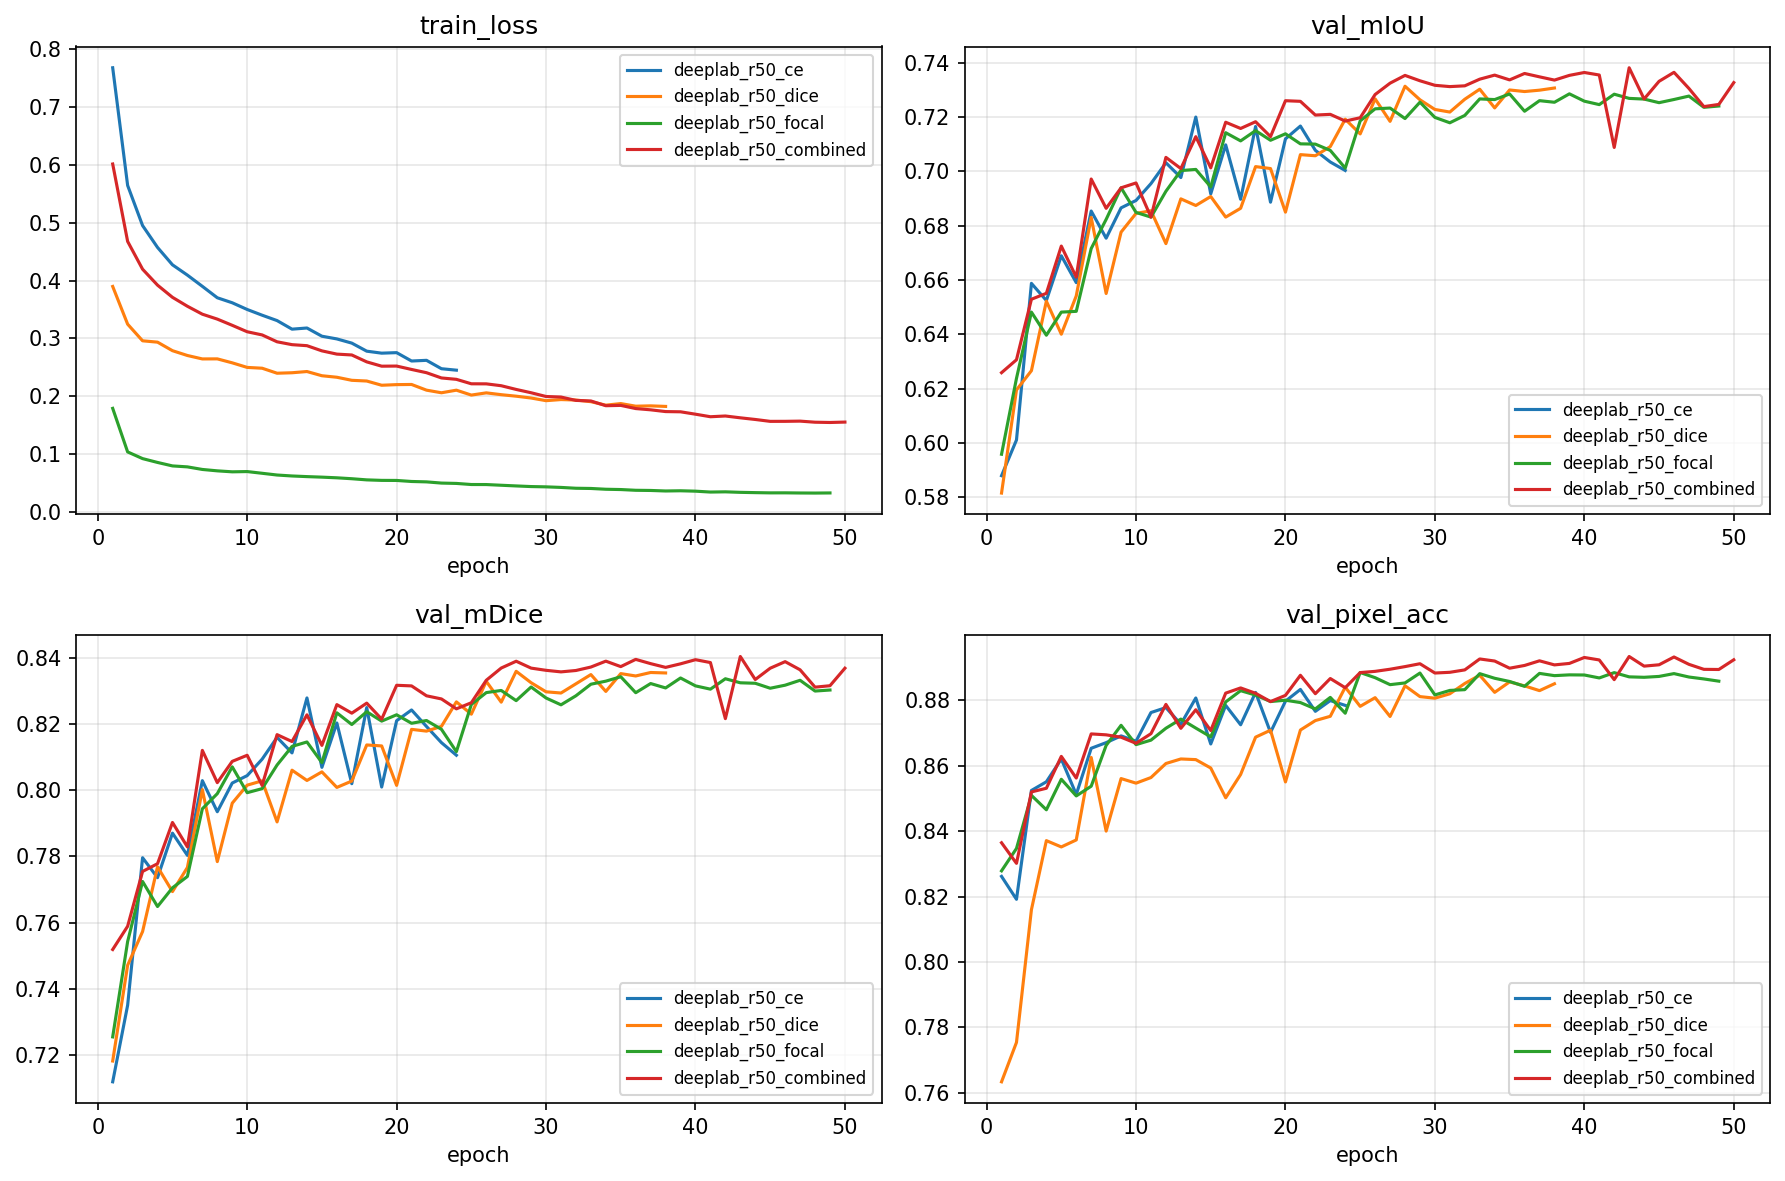
\includegraphics[width=\linewidth]{figs/curves_losses.png}
  \caption{Training / validation curves.}
\end{subfigure}\hfill
\begin{subfigure}[t]{0.40\linewidth}
  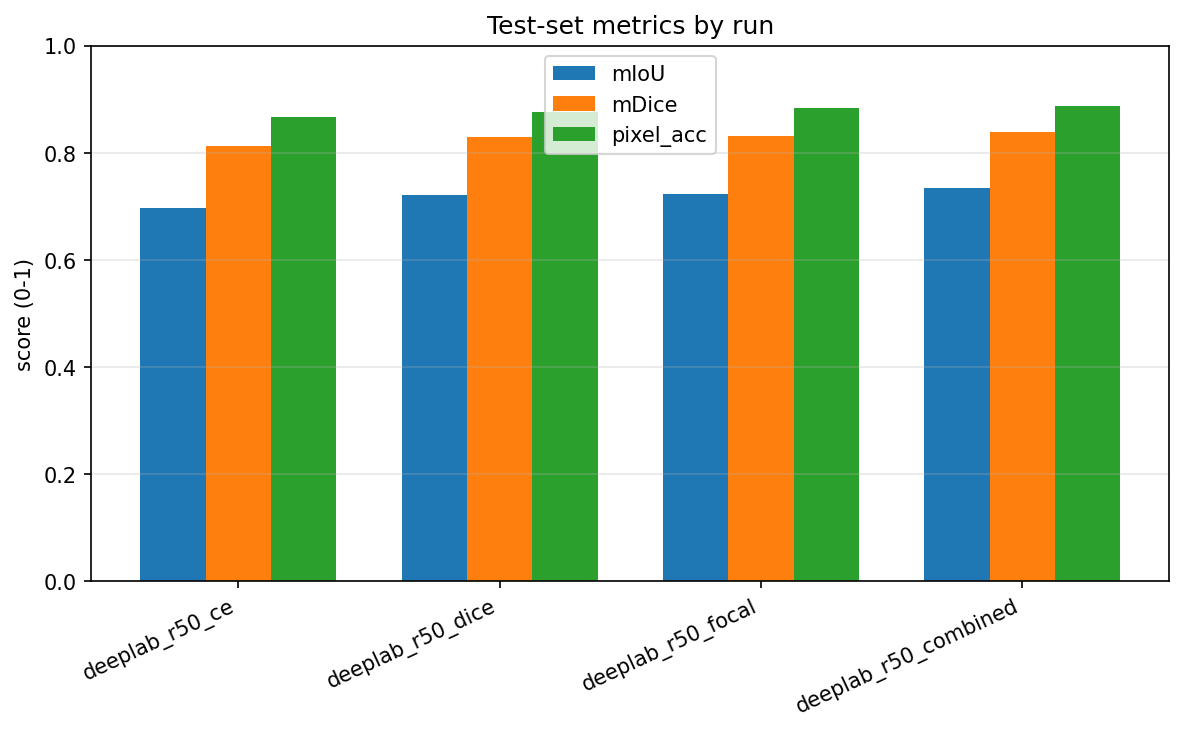
\includegraphics[width=\linewidth]{figs/losses_metrics.png}
  \caption{Final aggregate metrics.}
\end{subfigure}
\caption{Phase 5: loss-function comparison on DeepLabV3+-R50.}
\label{fig:loss-curves}
\end{figure*}

The most consequential finding is minority-class recovery: using the
Combined loss, the test Barren IoU rises from the CE baseline's 0.656
to 0.676, and---when comparing against the weakest (Vanilla U-Net + CE)
configuration---from 0.571 to 0.676, a \textbf{10.5 absolute-point}
improvement on one of the two rarest non-ignored classes (Barren,
Fig.~\ref{fig:classdist}). The Rangeland IoU, which is the hardest class
across all experiments, also improves from 0.415 to 0.454 (+9.4\%).
Overall mean test mIoU rises from 0.6963 to 0.7332. Focal and Dice each
individually beat CE by a smaller margin but fall short of the combination.

Figure~\ref{fig:cm} shows normalized confusion matrices for Attention
U-Net~+~CE (Phase 4 winner) and DeepLabV3+-R50~+~Combined (Phase 5
winner). Both models share a dominant failure mode: Rangeland pixels are
most often misclassified as \emph{Agriculture} (row fraction
$\sim 0.21$--$0.23$), with a smaller fraction confused with Forest
($\sim 0.02$--$0.03$). This is consistent with the visual similarity
between low-density rangeland and managed farmland in RGB satellite
imagery.

\begin{figure*}[!t]
\centering
\begin{subfigure}[t]{0.49\linewidth}
  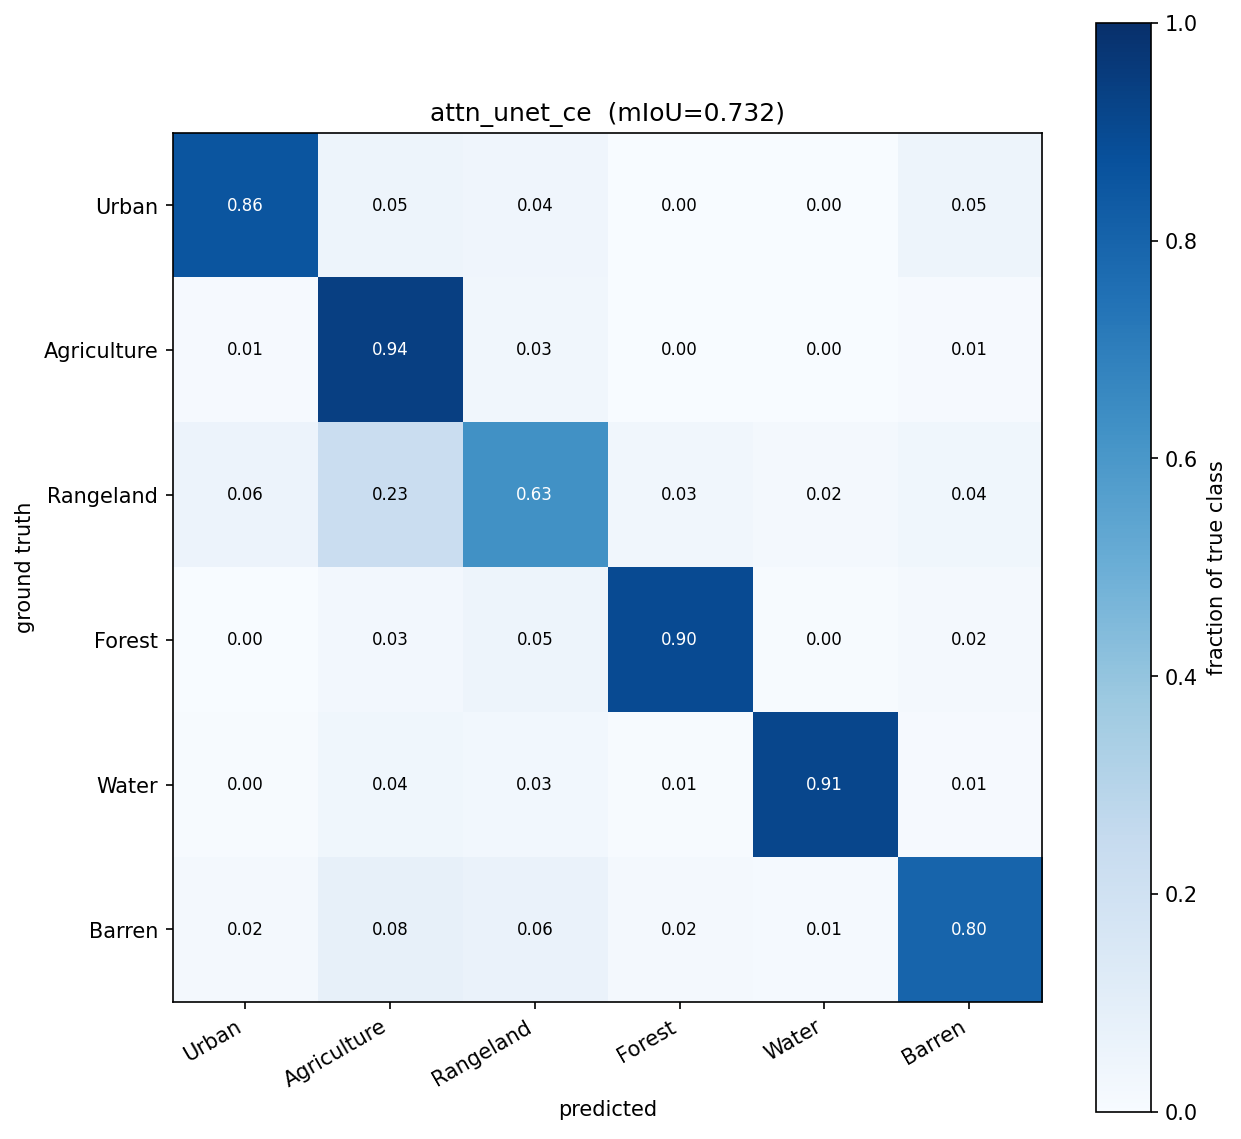
\includegraphics[width=\linewidth]{figs/cm_attn_unet_ce.png}
  \caption{Attention U-Net + CE.}
\end{subfigure}\hfill
\begin{subfigure}[t]{0.49\linewidth}
  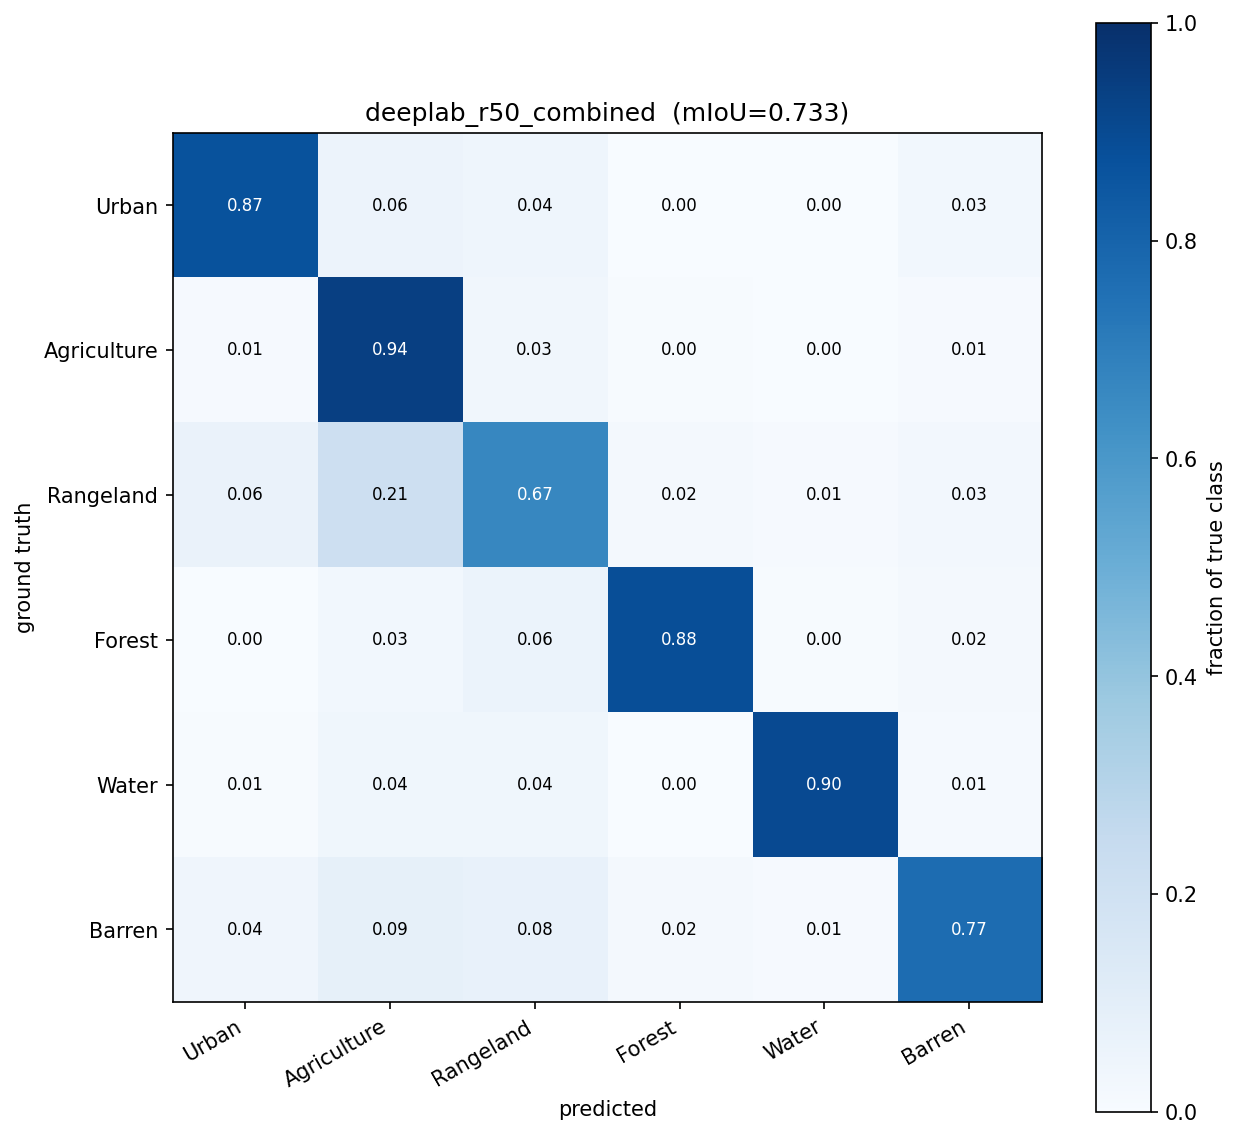
\includegraphics[width=\linewidth]{figs/cm_deeplab_r50_combined.png}
  \caption{DeepLabV3+-R50 + Combined.}
\end{subfigure}
\caption{Row-normalized confusion matrices (diagonal = per-class recall).}
\label{fig:cm}
\end{figure*}

\subsection{Qualitative and failure-case analysis}

Figure~\ref{fig:qual} shows side-by-side predictions from the three
strongest pipelines on three representative test scenes.
Figure~\ref{fig:failures} shows the five worst-performing test images of
the overall best model (DeepLabV3+-R50~+~Combined). In the failure
panels, the common error modes are (i) large Rangeland patches
predicted as Agriculture (the dominant confusion pair in
Fig.~\ref{fig:cm}), (ii) urban shadows classified as Water, and (iii)
bare-earth regions at agricultural boundaries classified as Barren.
Errors are concentrated at semantic transitions rather than in
homogeneous regions, which matches the intuition that the 816-pixel
tile receptive field is large enough for texture but sometimes too small
for global land-use disambiguation.

\begin{figure*}[!t]
\centering
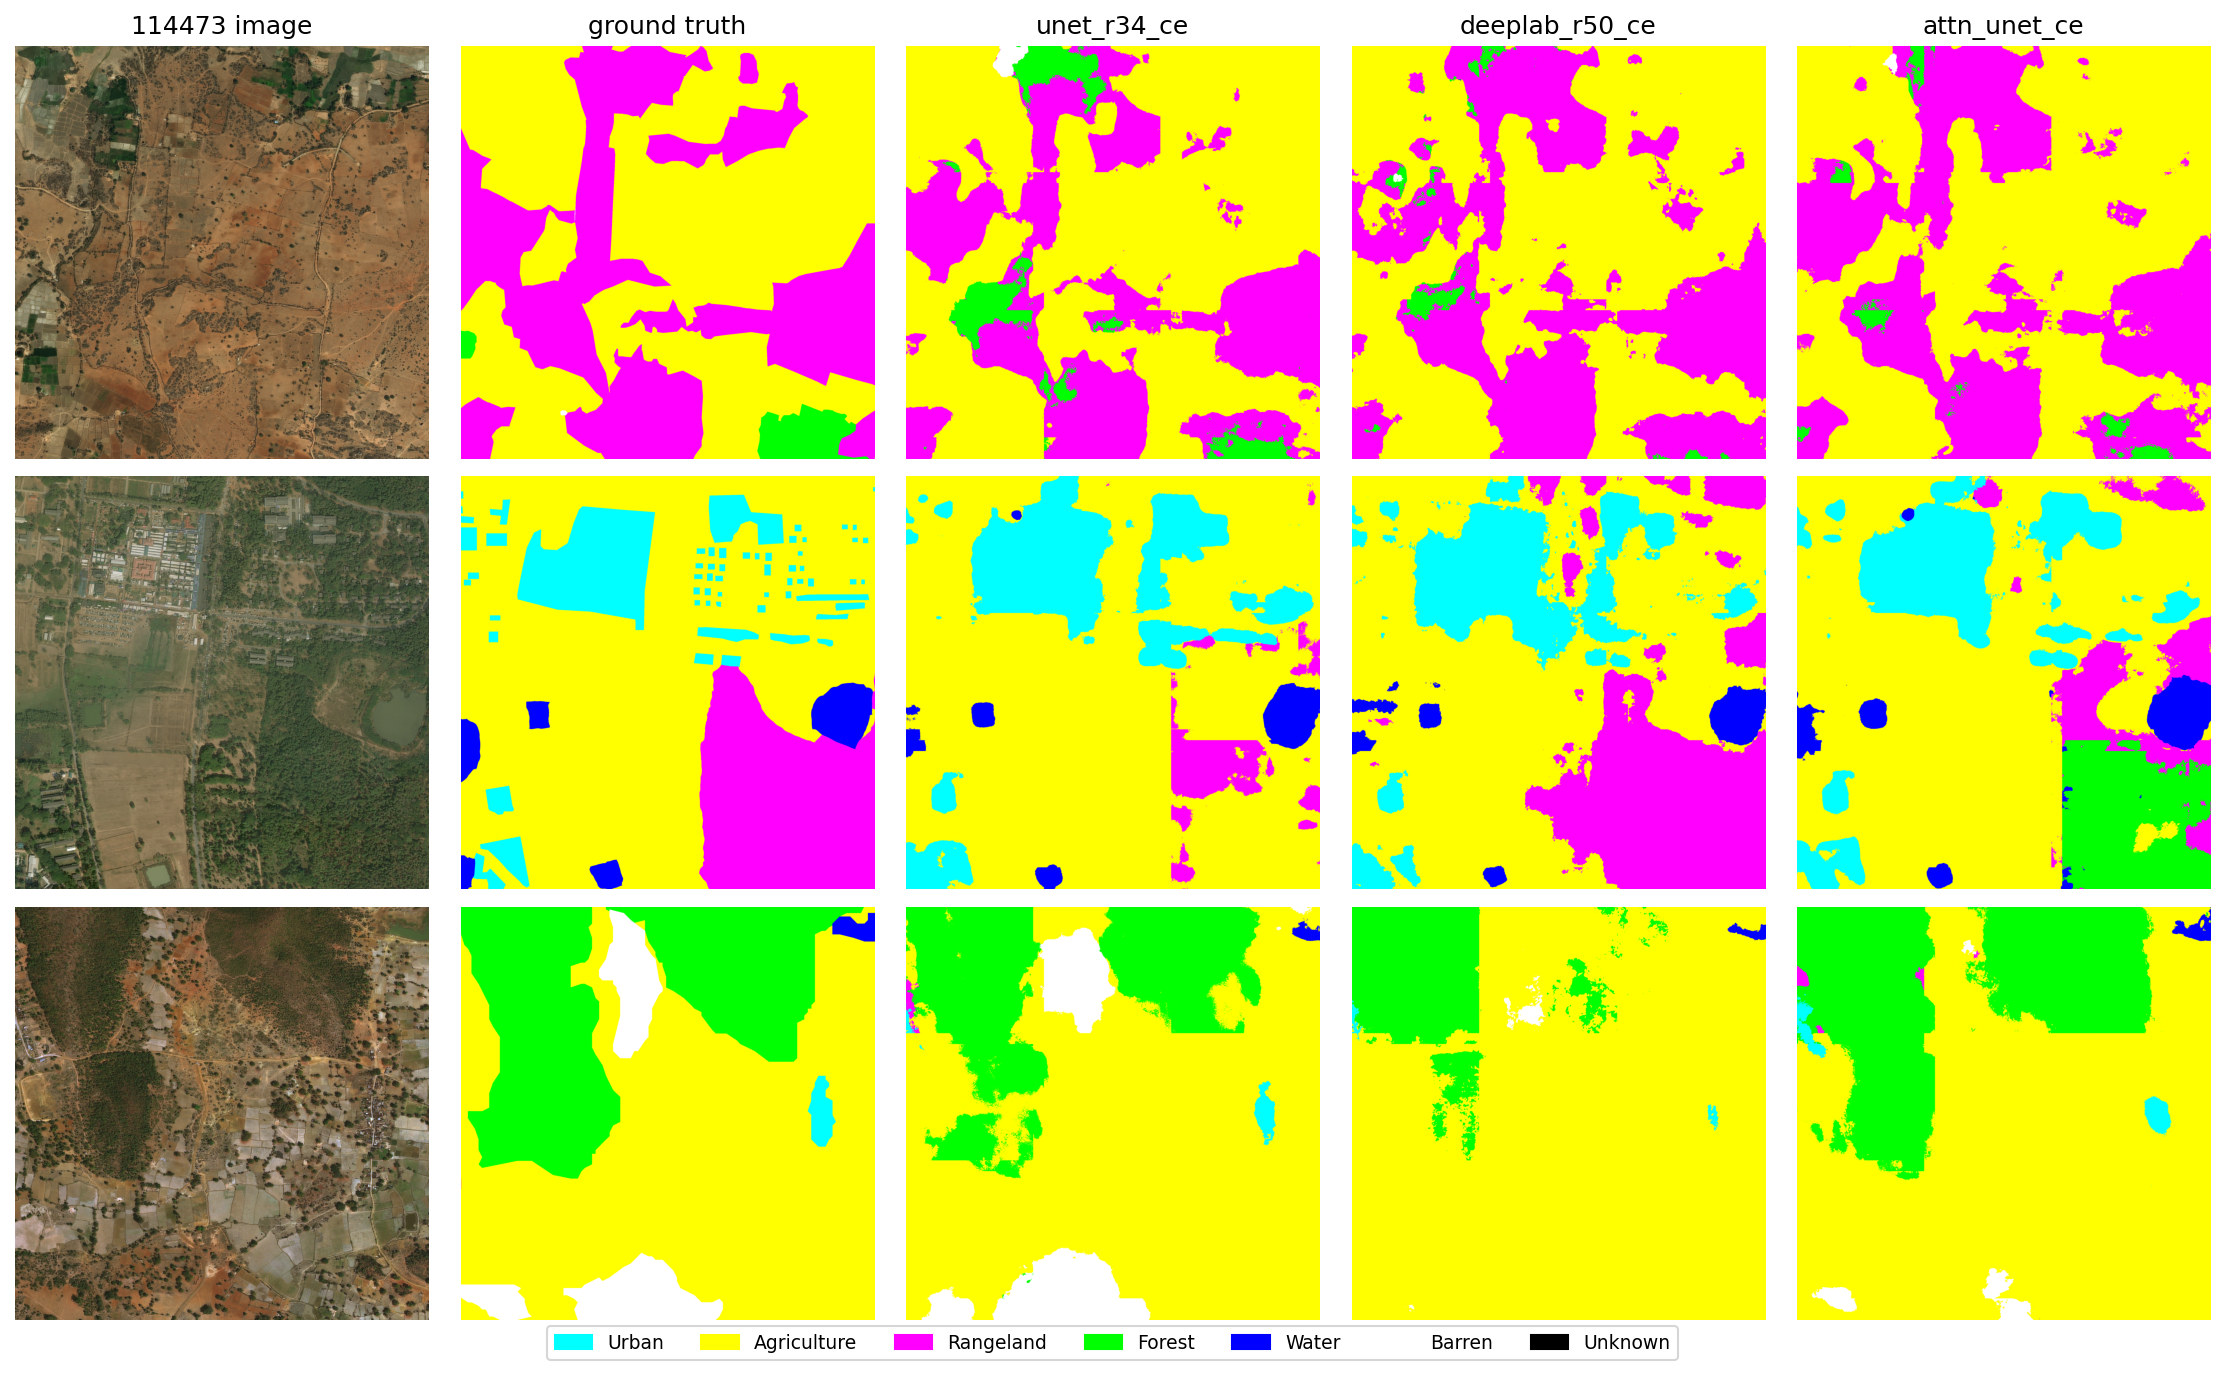
\includegraphics[width=\linewidth]{figs/qualitative.png}
\caption{Qualitative comparison on three test scenes: image, ground
truth, and predictions from three pipelines.}
\label{fig:qual}
\end{figure*}

\begin{figure*}[!t]
\centering
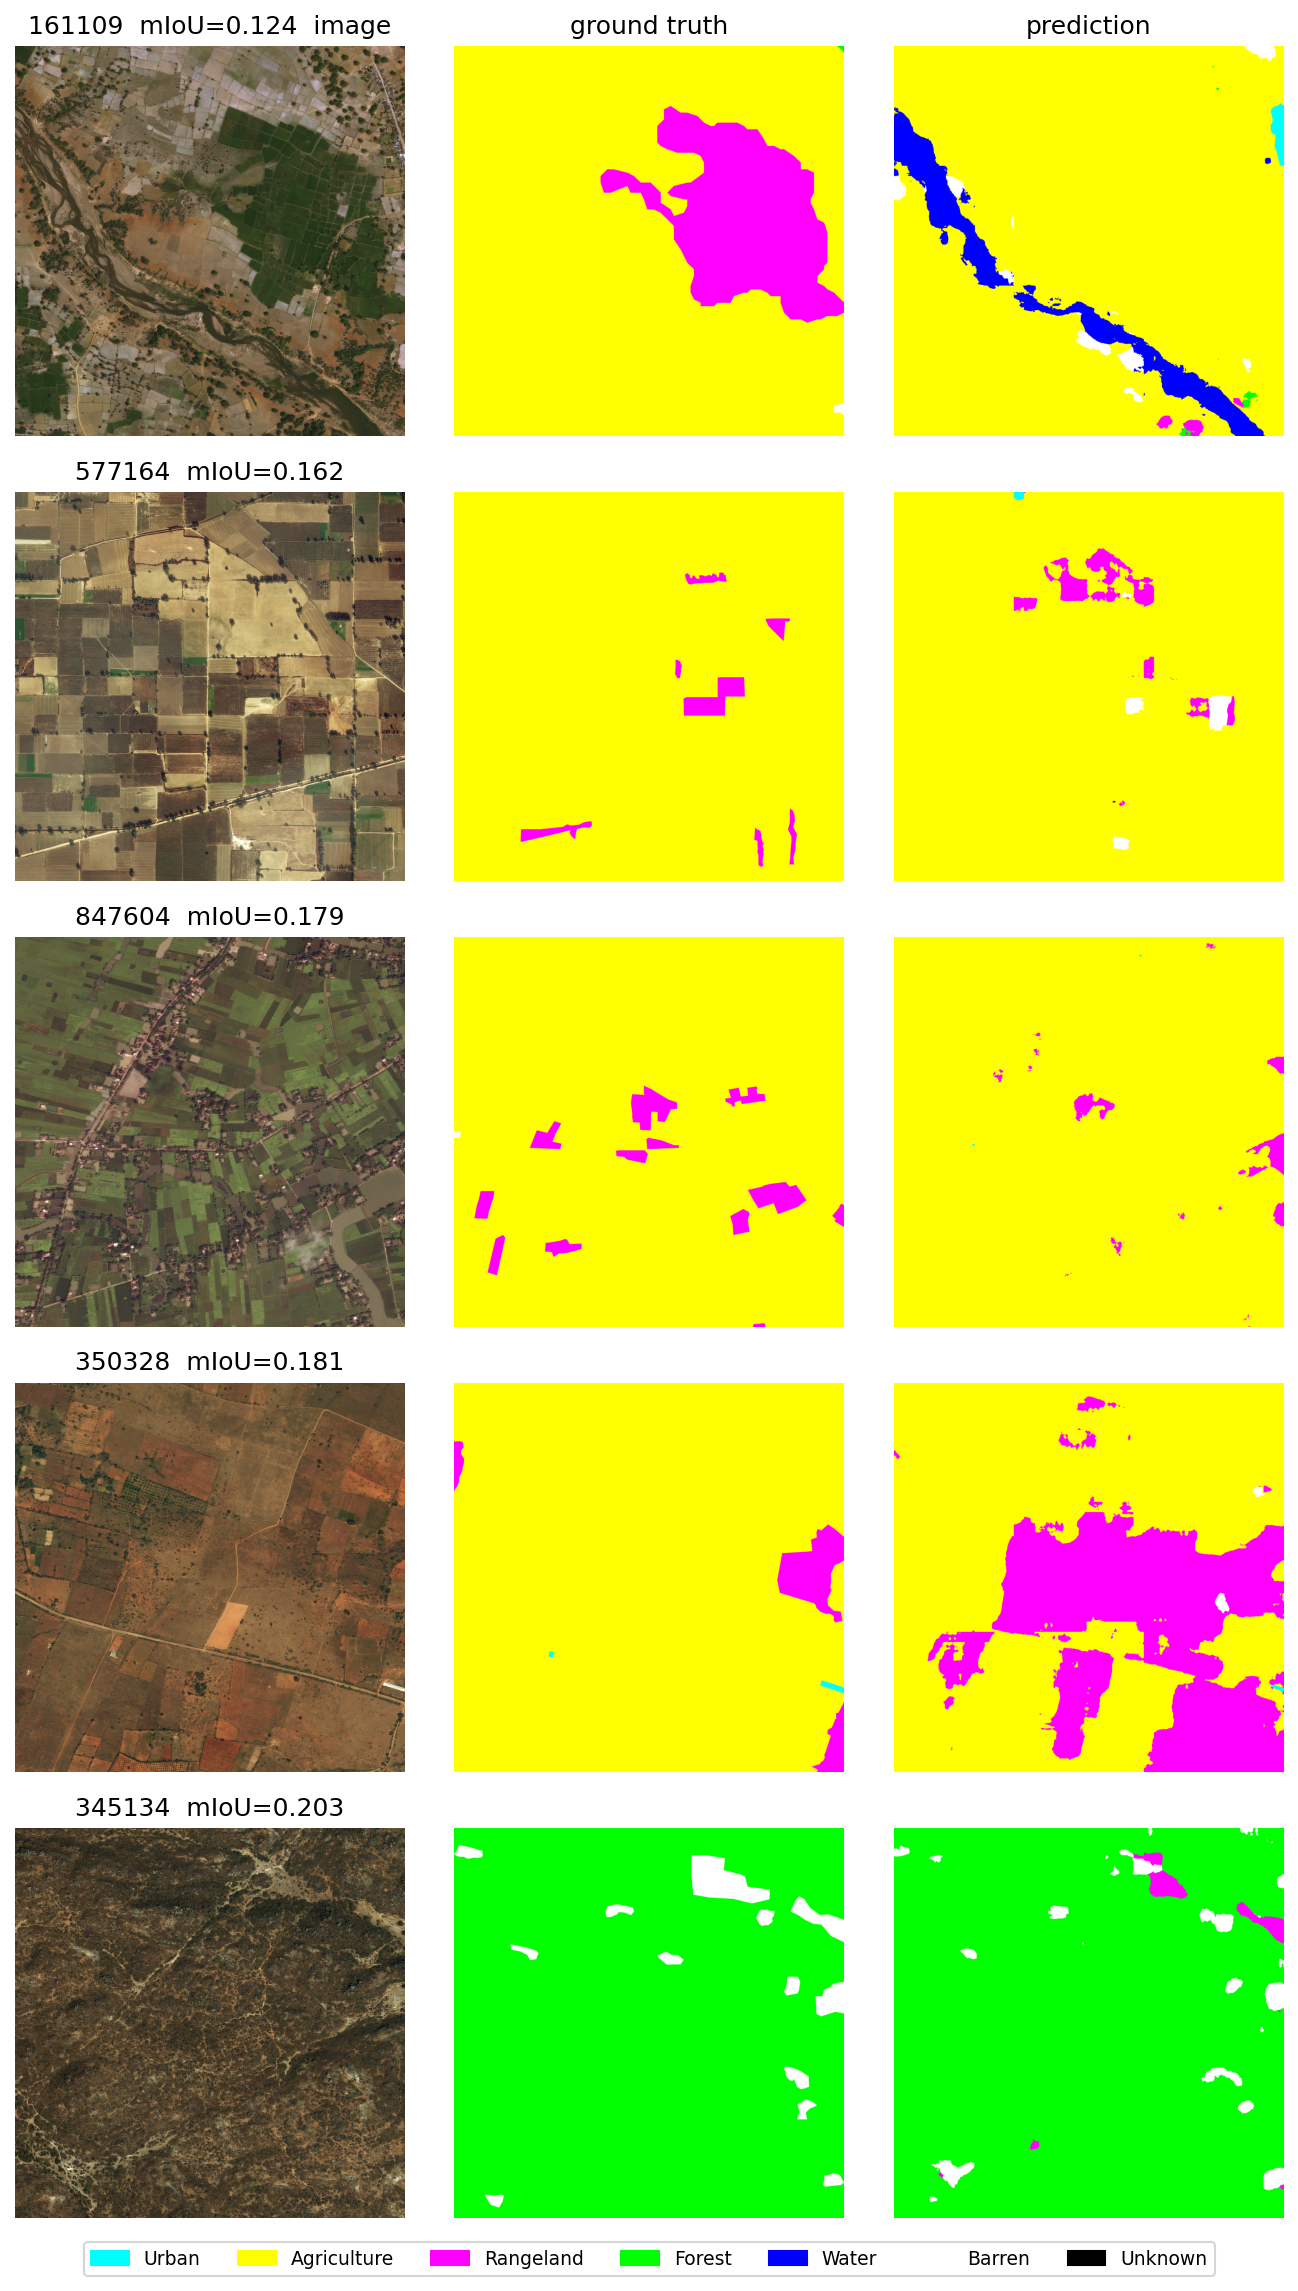
\includegraphics[height=0.85\textheight,keepaspectratio]{figs/failures_combined.png}
\caption{Five worst-performing test images for
DeepLabV3+-R50~+~Combined, ranked by test mIoU ascending. Misclassifications
cluster at semantic boundaries.}
\label{fig:failures}
\end{figure*}

\subsection{Efficiency vs.~accuracy}

The results also speak to cost-accuracy trade-offs. DeepLabV3+-R50 reaches
a validation mIoU within 0.006 of the best (Attention U-Net) while
training 2.3$\times$ faster and using comparable GPU memory. ResNet101
is \emph{not} Pareto-dominant against ResNet50: its test mIoU is
marginally higher ($+0.022$) but val mIoU is lower ($-0.008$)---both
within single-seed noise---while training and inference are
strictly worse (2.4$\times$ longer training, 53~ms/image slower).
Vanilla U-Net has the largest parameter count (31.0M) yet the lowest
accuracy, suggesting that for this task the encoder's inductive biases
and ImageNet pre-training matter more than raw capacity.

\section{Conclusions and Limitations}\label{sec:conclusion}

We presented nine controlled experiments on DeepGlobe Land Cover
Segmentation, isolating the effects of architecture, pre-training, and
loss function. Our three central findings are:

\begin{enumerate}
\item \textbf{Pre-training is the dominant single-variable factor.}
      Holding the architecture fixed at U-Net + ResNet34, switching from
      random initialization to ImageNet weights adds $+4.1$ pp mIoU.
      Among pretrained models, swapping the decoder
      (U-Net $\to$ DeepLabV3+ $\to$ Attention U-Net) adds at most
      $+1.0$ pp. The combined upgrade from Vanilla U-Net (scratch) to
      Attention U-Net (ImageNet) yields $+8.2$ pp on validation.
\item \textbf{Combined CE~+~Dice loss is the most effective defense
      against class imbalance} in our setting. Holding the architecture
      at DeepLabV3+-R50, the loss-only swap (CE $\to$ Combined) raises
      Barren test IoU by $+2.0$ pp and mean test IoU by $+3.7$ pp.
      Stacking the loss improvement on top of the architecture upgrade
      yields the full $+10.5$ pp Barren IoU over the Vanilla U-Net + CE
      baseline.
\item \textbf{Deeper encoders do not automatically win.}
      DeepLabV3+-R101 uses $71\%$ more parameters than R50 yet
      \emph{underperforms R50 on the validation set by $-0.008$ mIoU};
      on the test set it marginally exceeds R50 by $+0.022$, but with
      $2.4\times$ the training time and $\sim 6\%$ higher inference
      latency. At DeepGlobe's data scale, R101's extra capacity is not
      Pareto-optimal against R50.
\end{enumerate}

\textbf{Best configuration tested.} DeepLabV3+-R50 with Combined loss
achieves a test mIoU of \textbf{0.7332} on the full-resolution
reconstructed 120-image test set, exceeding the proposal's $\ge 0.55$
success threshold by $+18$ pp and the weakest in-study baseline
(Vanilla U-Net + CE at 0.6402) by $+9.3$ pp. We note that the combination
of Attention U-Net + Combined loss was not run and cannot be ruled out
as a stronger configuration.

\textbf{Limitations.} This study uses a single dataset (DeepGlobe); the
transfer-learning findings may not generalize to tasks with larger
domain gaps from ImageNet. We do not evaluate Transformer backbones
(Swin, SegFormer) which could change the encoder ranking. We did not
conduct full class-frequency-weighted loss experiments, which may
further improve minority-class performance. Finally, inference in this
project is tile-based; future work should compare against a full-image
Transformer that avoids tile-boundary artifacts altogether.

\textbf{Reproducibility.} All code, configurations, trained weights,
and per-epoch training logs are available at
\url{https://github.com/Jerryzhang258/landcover-seg}. The experiment
sweep is reproducible in $\sim$15 GPU-hours on an A100 through the
notebook \texttt{notebooks/colab\_run.ipynb}.

\begin{thebibliography}{00}

\bibitem{demir2018deepglobe}
I.~Demir, K.~Koperski, D.~Lindenbaum, G.~Pang, J.~Huang, S.~Basu, F.~Hughes,
D.~Tuia, and R.~Raskar, ``DeepGlobe 2018: A challenge to parse the Earth
through satellite images,'' in \emph{Proc. IEEE Conf. Comput. Vis. Pattern
Recognit. Workshops (CVPRW)}, Jun. 2018, pp. 172--181.

\bibitem{ronneberger2015unet}
O.~Ronneberger, P.~Fischer, and T.~Brox, ``U-Net: Convolutional networks
for biomedical image segmentation,'' in \emph{Proc. Int. Conf. Med. Image
Comput. Comput.-Assisted Intervention (MICCAI)}, 2015, pp. 234--241.

\bibitem{chen2018deeplabv3plus}
L.-C.~Chen, Y.~Zhu, G.~Papandreou, F.~Schroff, and H.~Adam, ``Encoder-decoder
with atrous separable convolution for semantic image segmentation,''
in \emph{Proc. Eur. Conf. Comput. Vis. (ECCV)}, 2018, pp. 801--818.

\bibitem{roy2018scse}
A.~G.~Roy, N.~Navab, and C.~Wachinger, ``Concurrent spatial and channel
squeeze-and-excitation in fully convolutional networks,'' in \emph{Proc.
Int. Conf. Med. Image Comput. Comput.-Assisted Intervention (MICCAI)},
2018, pp. 421--429.

\bibitem{he2016resnet}
K.~He, X.~Zhang, S.~Ren, and J.~Sun, ``Deep residual learning for image
recognition,'' in \emph{Proc. IEEE Conf. Comput. Vis. Pattern Recognit.
(CVPR)}, Jun. 2016, pp. 770--778.

\bibitem{huh2016makes}
M.~Huh, P.~Agrawal, and A.~A.~Efros, ``What makes ImageNet good for
transfer learning?'' \emph{arXiv preprint}, arXiv:1608.08614, 2016.

\bibitem{milletari2016vnet}
F.~Milletari, N.~Navab, and S.-A.~Ahmadi, ``V-Net: Fully convolutional
neural networks for volumetric medical image segmentation,'' in
\emph{Proc. Int. Conf. 3D Vis. (3DV)}, 2016, pp. 565--571.

\bibitem{lin2017focal}
T.-Y.~Lin, P.~Goyal, R.~Girshick, K.~He, and P.~Doll\'ar, ``Focal loss
for dense object detection,'' in \emph{Proc. IEEE Int. Conf. Comput. Vis.
(ICCV)}, Oct. 2017, pp. 2980--2988.

\bibitem{jadon2020survey}
S.~Jadon, ``A survey of loss functions for semantic segmentation,''
in \emph{Proc. IEEE Conf. Comput. Intell. Bioinform. Comput. Biol.
(CIBCB)}, 2020, pp. 1--7.

\bibitem{kuo2018deepglobewinner}
T.-S.~Kuo, K.-S.~Tseng, J.-W.~Yan, Y.-C.~Liu, and Y.-C.~F.~Wang,
``Deep aggregation net for land cover classification,'' in
\emph{Proc. IEEE Conf. Comput. Vis. Pattern Recognit. Workshops (CVPRW)},
Jun. 2018, pp. 252--256.

\bibitem{roerdink2001watershed}
J.~B.~T.~M.~Roerdink and A.~Meijster, ``The watershed transform:
Definitions, algorithms and parallelization strategies,''
\emph{Fundamenta Informaticae}, vol.~41, no. 1--2, pp. 187--228, 2000.

\bibitem{huang2021transunet}
J.~Chen, Y.~Lu, Q.~Yu, X.~Luo, E.~Adeli, Y.~Wang, L.~Lu, A.~Yuille, and
Y.~Zhou, ``TransUNet: Transformers make strong encoders for medical image
segmentation,'' \emph{arXiv preprint}, arXiv:2102.04306, 2021.

\bibitem{iakubovskii2019smp}
P.~Iakubovskii, ``Segmentation Models PyTorch,'' GitHub repository, 2019.
[Online]. Available: \url{https://github.com/qubvel/segmentation_models.pytorch}

\end{thebibliography}

\end{document}
